\documentclass{article}
\usepackage{amsmath}
\usepackage{amssymb}
\usepackage{graphicx}
\usepackage{hyperref}
\usepackage[version=4]{mhchem}

\title{Problem 1}
\date{}

\begin{document}
\maketitle

\section*{Problem}
(AMC) Let line \(A C\) be perpendicular to line \(C E\). Connect \(A\) to the midpoint \(D\) of \(C E\), and connect \(E\) to the midpoint \(B\) of \(A C\). If \(A D\) and \(E B\) intersect in point \(F\), and \(B C=C D=15\) inches, find the area of triangle \(D F E\) in square inches.

\section*{Solution}
(C).\\
Method 1 (official solution):\\
Draw \(A E\) and the altitude \(F G\) to the base \(D E\) of triangle \(D E F\). Since \(F\) is the intersection point of the medians of a triangle \(A C E, F D=\frac{1}{3} A D\).\\
\(\therefore F G=\frac{1}{3} A C=\frac{1}{3} \cdot 30=10\).\\
\centering
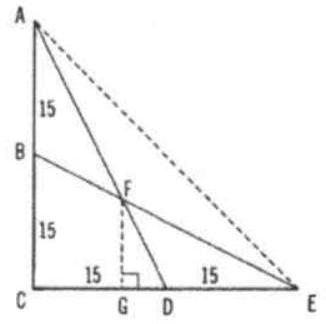
\includegraphics[width=\textwidth]{images/problem_image_1.jpg}\\
\(\therefore \operatorname{area}(\triangle D E F)=\frac{1}{2} \cdot 15 \cdot 10=75\).\\
The three medians of a triangle divide the triangle into six triangles of equal area. Therefore, \(\operatorname{Area}(\triangle F D E)=75\).

Method 2 (our solution):\\
Connect \(A E\). Then connect \(C F\) and extend it to meet \(A E\) at \(M\). \(F\) is the centroid and triangle \(A C E\) is divided into six smaller triangles with the same area.\\
The area of \((\triangle A C D)=\frac{1}{2} \cdot 30 \cdot 15=225\). The area of\\
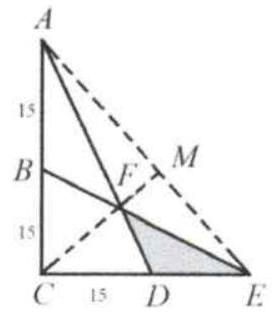
\includegraphics[width=\textwidth]{images/reasoning_image_1.jpg} \((\triangle F D E)=\frac{225}{3}=75\).

\end{document}
